% !TEX root = ./main.tex
% !TEX encoding = UTF-8 Unicode
% !TEX program = pdflatex
% !TeX spellcheck = en_GB

\chapter{Scelta Architetturale}
In questo capito sarà mostrata l'architettura del sistema utilizzato per
la risoluzione del problema di Influence Maximization. Il sistema è formato da un
livello di data storage e un livello di elaborazione.

\section{MongoDB}
Nel livello dati del sistema, come da requisiti, si richiede l'utilizzo di un database
noSql. Esistono diversi tipi di database noSql, tra cui: chiave-valore, colonnari,
graph-db e documentali. Nel caso in esame, dopo aver visionato i dati a nostra
disposizione, si scelto un database documentale, in particolare \textit{\textbf{MongoDB}}.
I database documentali sono adatti alla memorizzazione di dati aggregati, ma non
adatti all'esecuzione di quary complesse. Infatti in tali database ogni record è visto
come un documento contente delle caratteristiche, l'accesso ad ogni documento
può essere effettuato solo tramite una chiave. Poiché i nostri dati sono
memorizzati in file .json  presentando strutture dati non elementare, come ad
esempio il campo \textit{Elite} del file utenti, ed inoltre è stato scelto di non
effettuare pressing dei dati nel livello database la scelta è ricaduta su questo
tipo di db. MongoDB è stato installato per fini didattici su di un singolo nodo, di seguito
saranno riportati i dettagli.
\begin{figure}[!htbp]
	
\includegraphics[width=.7\linewidth,keepaspectratio]{mongo.png}
  \caption{MongoDB}
  \label{}
\end{figure}
\section{Apache Spark}
Apache Spark è un framework open source per il calcolo distribuito. Utilizza il
paradigma MapReduce in memory riuscendo a raggiungere prestazioni 100 volte superiori
a quelle raggiunte da Hadoop. Tale framework è disponibile nei seguenti linguaggi di
programmazione: \textit{\textbf{Scala}}, \textit{\textbf{Java}}, \textit{\textbf{Python}}
e \textit{\textbf{R}}.
Inoltre per poter creare il grafo si è fatto uso del framework Graphx, il quale
rende disponibili diversi metodi applicabili su grafi. Per poter utilizzare
Apache Spark  si è utilizzata la piattaforma cloud Databrick la quale rende
disponibile in versione community un cluster composto da 8 core e 6GB di RAM.
\begin{figure}[!htbp]
	
\includegraphics[width=.7\linewidth,keepaspectratio]{spark.png}
  \caption{Apache Spark}
  \label{}
\end{figure}

\clearpage

\section{Archittettura}
Quindi in definitiva il sistema scelto è cosi formato:
\begin{itemize}
	\item MongoDB per lo storage dei dati di origine e per dei risultati;
	\item Apache Spark per il pre-processing dei dati;
	\item Graphx la creazione del grafo e per l'implementazione dell'algoritmo di Influence
	Maximization.
\end{itemize}
Nella seguente figura è mostato l'architettura utilizzata.
\begin{figure}[!htbp]
	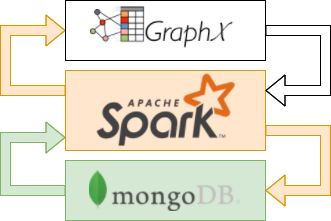
\includegraphics[width=.7\linewidth,keepaspectratio]{architettura.png}
  \caption{Archiettura del sistema}
  \label{sysarch}
\end{figure}
Quindi in definitiva MongoDB risiede su di un nodo mentre Apache Spark con Graphx
è in Databricks.
